% Avance 2 · Detección de celdas solares defectuosas en imágenes EL · PDI 2026-III
% Compilar desde esta carpeta:  latexmk -pdf presentacion.tex
% Mismo estilo que la presentación de la propuesta. Figuras: reports/figures (generadas por los scripts).
\documentclass[aspectratio=169,11pt]{beamer}

\usepackage[T1]{fontenc}
\usepackage[utf8]{inputenc}
\usepackage{lmodern}
\usepackage[spanish,es-noshorthands,es-nodecimaldot]{babel}
\usepackage{amsmath,amssymb}
\usepackage{booktabs}
\usepackage{array}
\usepackage{tikz}
\usetikzlibrary{positioning,arrows.meta}

\graphicspath{{../../reports/figures/}{../comun/}}

% ------------------------------------------------------------------ estilo (igual a la propuesta)
\definecolor{ud}{RGB}{128,57,61}
\definecolor{udsoft}{RGB}{242,230,231}
\definecolor{tinta}{RGB}{64,64,64}
\definecolor{gris}{RGB}{120,120,120}
\definecolor{caja}{RGB}{244,244,244}
\definecolor{okc}{RGB}{27,140,96}

\usefonttheme{serif}
\setbeamertemplate{navigation symbols}{}
\setbeamercolor{normal text}{fg=tinta}
\setbeamercolor{structure}{fg=ud}
\setbeamercolor{alerted text}{fg=ud}
\setbeamerfont{frametitle}{size=\Large,series=\bfseries}
\setbeamerfont{framesubtitle}{size=\small}

\setbeamertemplate{frametitle}{%
  \vskip0.25cm
  \begin{beamercolorbox}[wd=\paperwidth,leftskip=-0.15cm]{frametitle}%
    \begin{minipage}[c]{1.75cm}\centering
\includegraphics[height=1.15cm]{logo.png}\end{minipage}%
    \hspace{0.35cm}%
    \begin{minipage}[c]{0.78\paperwidth}
      {\usebeamerfont{frametitle}\color{ud}\insertframetitle}\par
      {\usebeamerfont{framesubtitle}\mdseries\color{ud}\insertframesubtitle}
    \end{minipage}%
  \end{beamercolorbox}%
  \vskip0.1cm
}
\setbeamertemplate{footline}{%
  \hspace{0.45cm}{\color{gris}\scriptsize Avance 2 · Semana 2}\hfill{\color{gris}\scriptsize\insertframenumber}\hspace{0.45cm}\vspace{0.35cm}}
\setbeamertemplate{itemize item}{\color{ud}\raisebox{0.15ex}{\small$\bullet$}}
\setbeamertemplate{enumerate item}{\color{ud}\insertenumlabel.}
\setlength{\leftmargini}{1.4em}

\newcommand{\hecho}{{\color{okc}$\checkmark$}}
\newcommand{\cab}[1]{{\color{ud}\bfseries #1}\par\vspace{-2pt}{\color{ud}\rule{\linewidth}{0.4pt}}\par\vspace{2pt}}
% Recuadro con una cifra grande
\newcommand{\cifra}[3]{%
  \begin{tikzpicture}[baseline=(n.north)]\node(n)[draw=gray!45,fill=caja,rounded corners=1.5pt,minimum width=#1,minimum height=2.7cm,
     text width=#1-0.4cm,align=center,inner sep=5pt,anchor=north]{\parbox[t][2.35cm][t]{\dimexpr#1-0.4cm\relax}{\centering\rule{0pt}{0.45cm}{\color{ud}\fontsize{16}{19}\selectfont\mbox{#2}}\par\vspace{6pt}{\scriptsize #3\par}}};\end{tikzpicture}}

\title{Avance 2 · Quitar los busbars}
\date{25 de noviembre de 2026}

\setbeamertemplate{title page}{%
  \begin{tikzpicture}[remember picture,overlay]
    \node[anchor=south east,inner sep=0] at ([xshift=-0.2cm]current page.south east)
      {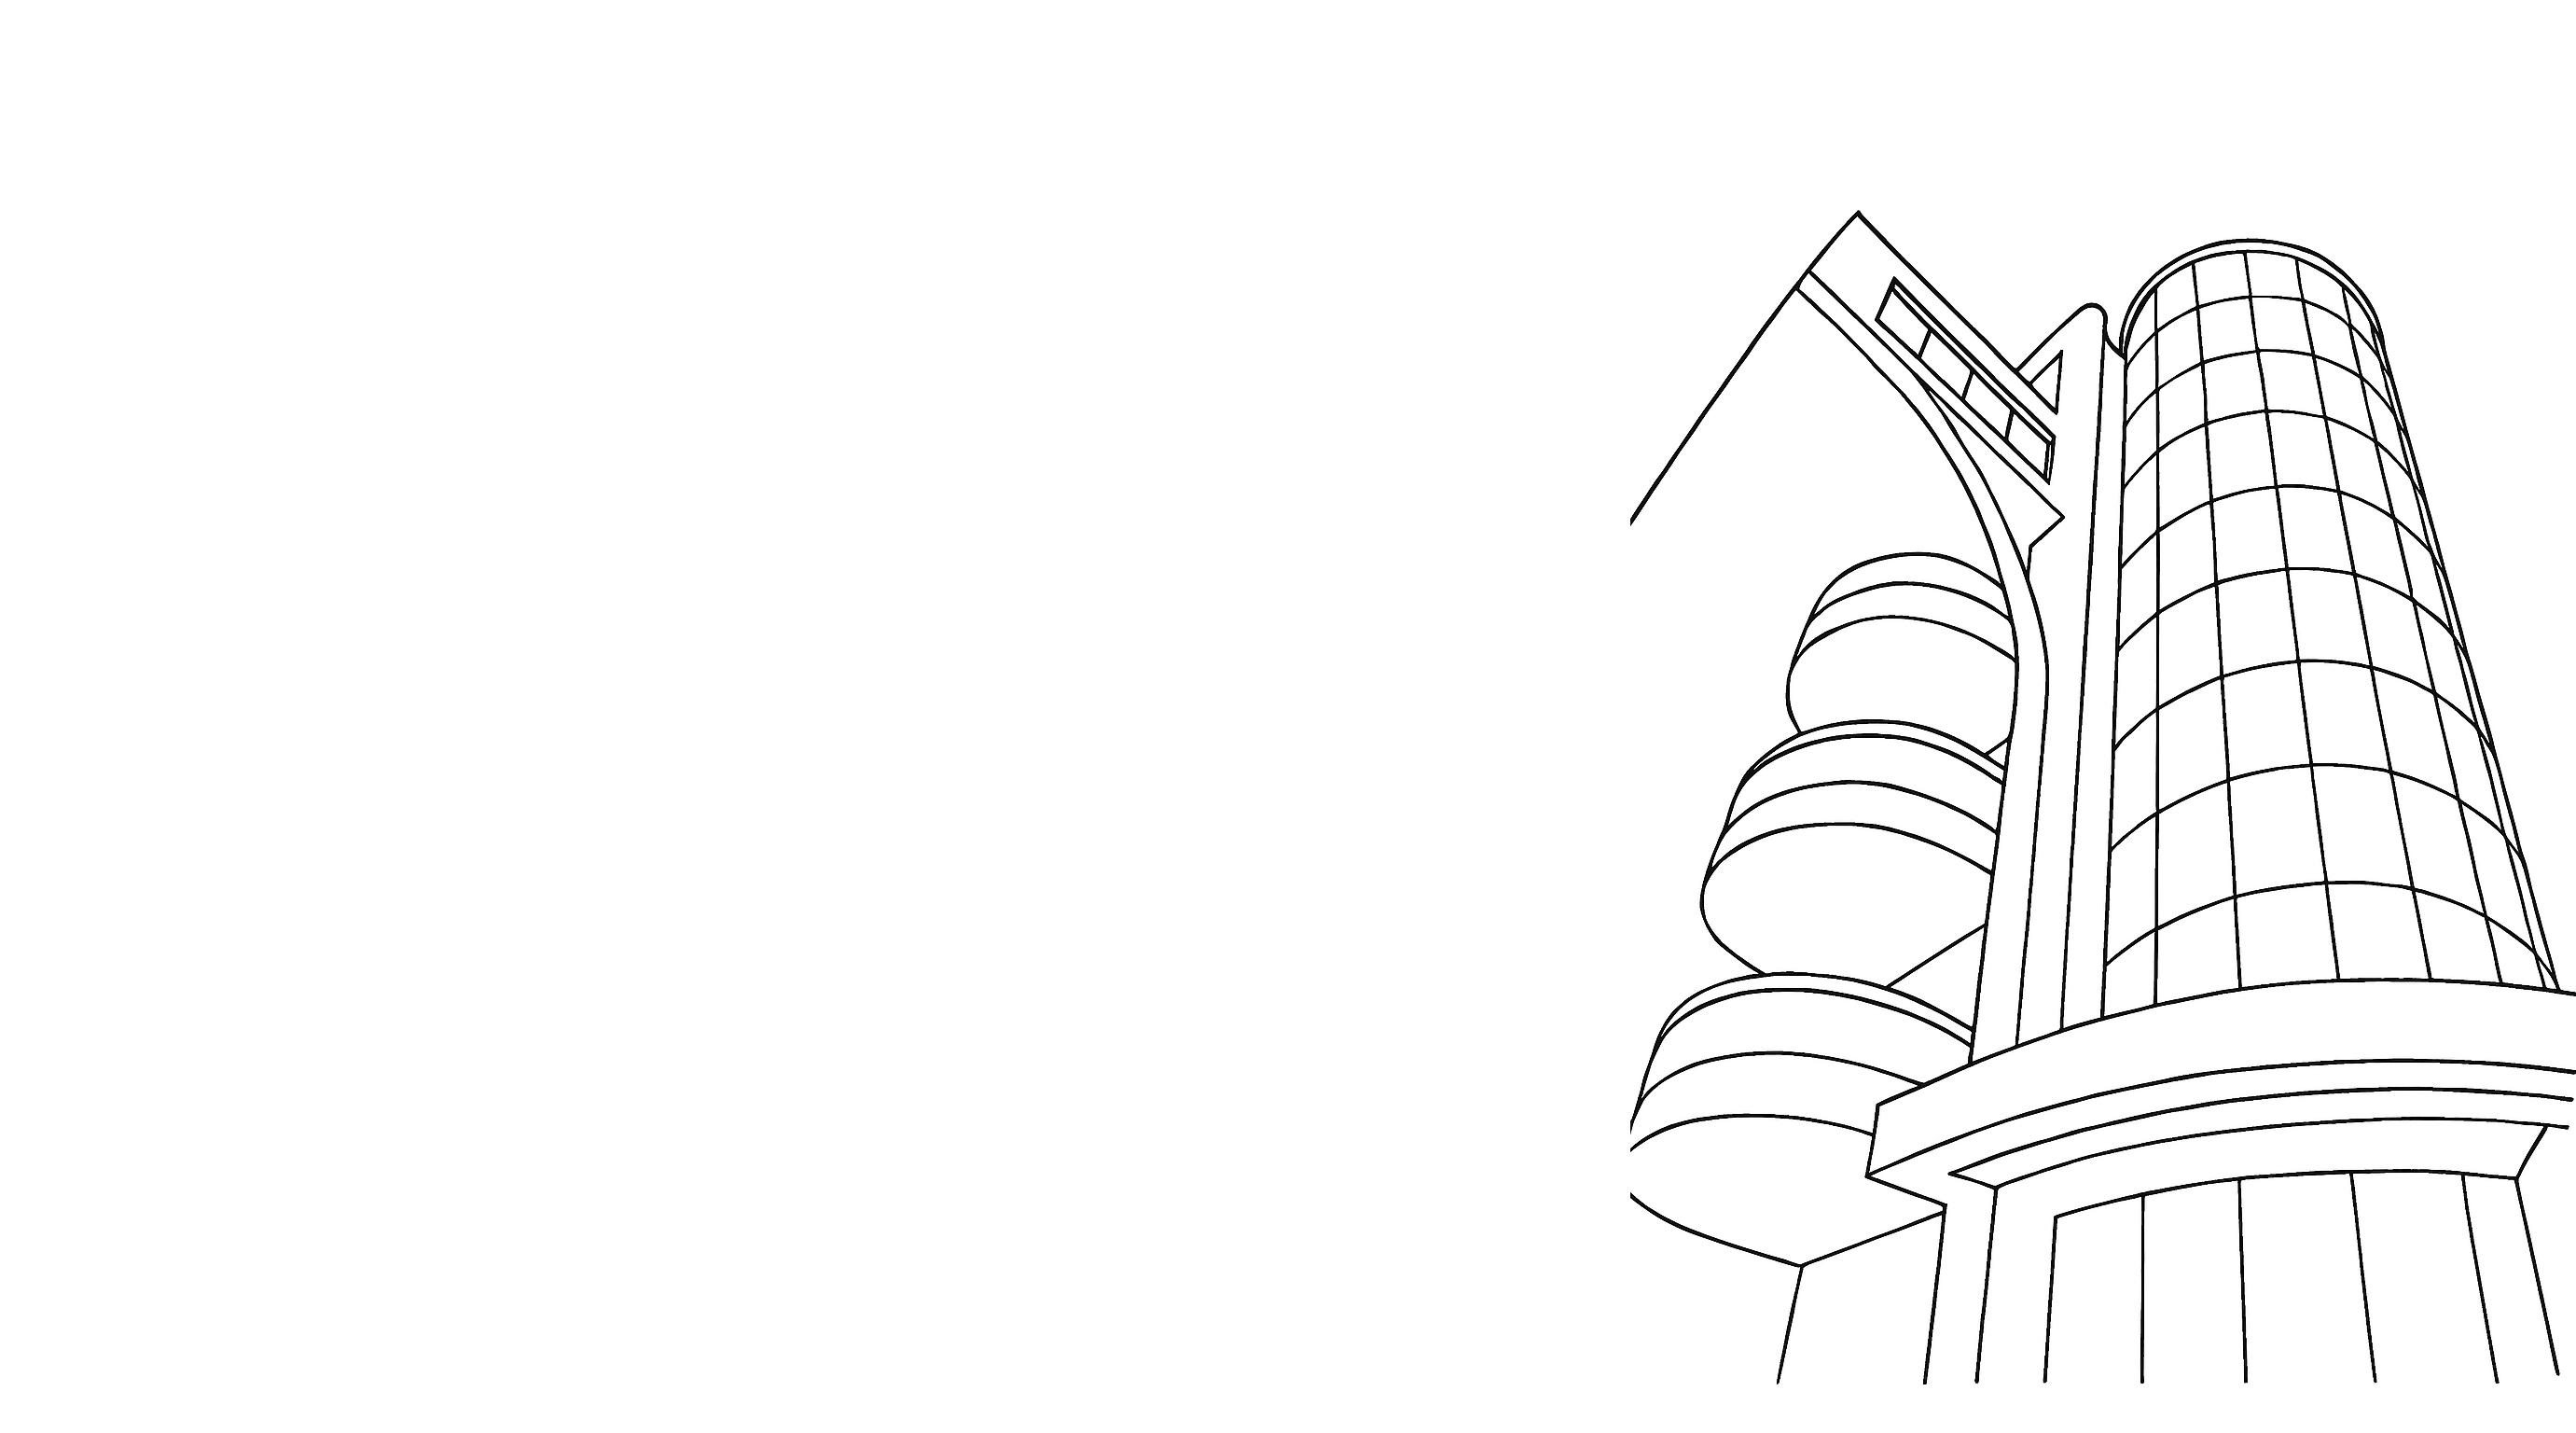
\includegraphics[height=0.97\paperheight]{edificio.png}};
    \node[anchor=north west] at ([xshift=0.6cm,yshift=-0.35cm]current page.north west)
      {
\includegraphics[height=1.3cm]{logo.png}};
  \end{tikzpicture}%
  \hbox{}\par\vspace{1.75cm}
  \begin{minipage}{0.6\textwidth}
    {\color{gris}\small AVANCE 2 · SEMANA 2 (16 – 22 DE NOVIEMBRE)}\par\vspace{0.2cm}
    {\color{ud}\Large\textsc{Quitar los busbars:\\ notch frente a cierre}}\par\vspace{0.3cm}
    {\color{ud}Detección de celdas solares defectuosas\\ en imágenes de electroluminiscencia\\ Procesamiento Digital de Imágenes · UD}\par\vspace{0.25cm}
    \small
    \begin{tabular}{@{}l@{\hspace{1.2em}}r@{}}
      Joel Eduardo Reyes Barrios & 20212005011\\
      Johan Sebastián Cáceres Rodríguez & 20212005111\\
      Hosman Javier Nieto Cruz & 20212005117
    \end{tabular}\par\vspace{0.3cm}
    25 de noviembre de 2026
  \end{minipage}
}

\begin{document}

\begin{frame}[plain,t]
  \titlepage
\end{frame}

\begin{frame}{La semana 2 en una diapositiva}{1 · Resumen}
  Las dos técnicas quitan los busbars. Se diferencian en lo que le hacen al resto de la celda.
  \vspace{0.25cm}

  \centering
  \cifra{3.2cm}{12$\,\rightarrow\,$100\,\%}{celdas de validación con la rejilla detectada exacta}\hfill
  \cifra{3.2cm}{0,9\,\%}{resto del busbar con el cierre (notch: 5,9\,\% global, 11,7\,\% en filas)}\hfill
  \cifra{3.2cm}{3\,\% \textit{vs.} 84\,\%}{contraste de una grieta a 45° que cruza un busbar: cierre y notch}\hfill
  \cifra{3.2cm}{$-40$\,\%}{respuesta de Sato de una grieta vertical fina al quitar dedos ($1\times3$)}

  \vspace{0.3cm}
  \raggedright
  \begin{itemize}
    \item \textbf{Decidido:} la detección v2 reemplaza a la v1.
    \item \textbf{Sin decidir:} notch o cierre. Lo decide el AUC de la CNN (criterio 3), en la semana 3.
    \item \textbf{Propuesta de cambio:} no quitar los dedos.
  \end{itemize}
\end{frame}

\begin{frame}{Semana 2: actividades técnicas hechas}{2 · Avance frente al cronograma}
  \small
  \begin{tabular}{@{}c p{7.4cm} p{5.6cm}@{}}
    \toprule
    & Actividad (tabla 6 de la propuesta) & Dónde quedó \\
    \midrule
    \hecho & Detección de busbars por celda & \texttt{src/busbars.py} \\
    \hecho & Notch (A-global, A-filas) y cierre (B) & \texttt{src/busbars.py} \\
    \hecho & Comparación en validación, criterios 1, 2 y 4 & \texttt{scripts/07\_\ldots} \\
    \hecho & Dedos y grietas verticales finas, con Sato & \texttt{scripts/09\_\ldots} \\
    \midrule
    {\color{ud}+} & Grietas sintéticas y página interactiva & \texttt{entregas/avance\_2/web} \\
    \bottomrule
  \end{tabular}

  \vspace{0.45cm}
  \begin{tikzpicture}[x=2.75cm]
    \foreach \i/\t in {1/Datos,2/Busbars,3/CNN,4/Prueba,5/Cierre} {
      \ifnum\i<3 \fill[ud] (\i-1,0) rectangle (\i-0.04,0.18); \else \fill[gray!30] (\i-1,0) rectangle (\i-0.04,0.18); \fi
      \node[anchor=north west,font=\footnotesize] at (\i-1,-0.05) {\textbf{S\i} · \t};
    }
    \draw[ud,very thick,dashed] (2.4,-0.55) -- (2.4,0.45) node[above,font=\scriptsize\bfseries,ud] {hoy};
  \end{tikzpicture}
\end{frame}

\begin{frame}{Qué es un busbar y qué es un dedo}{3 · Métodos}
  \centering
  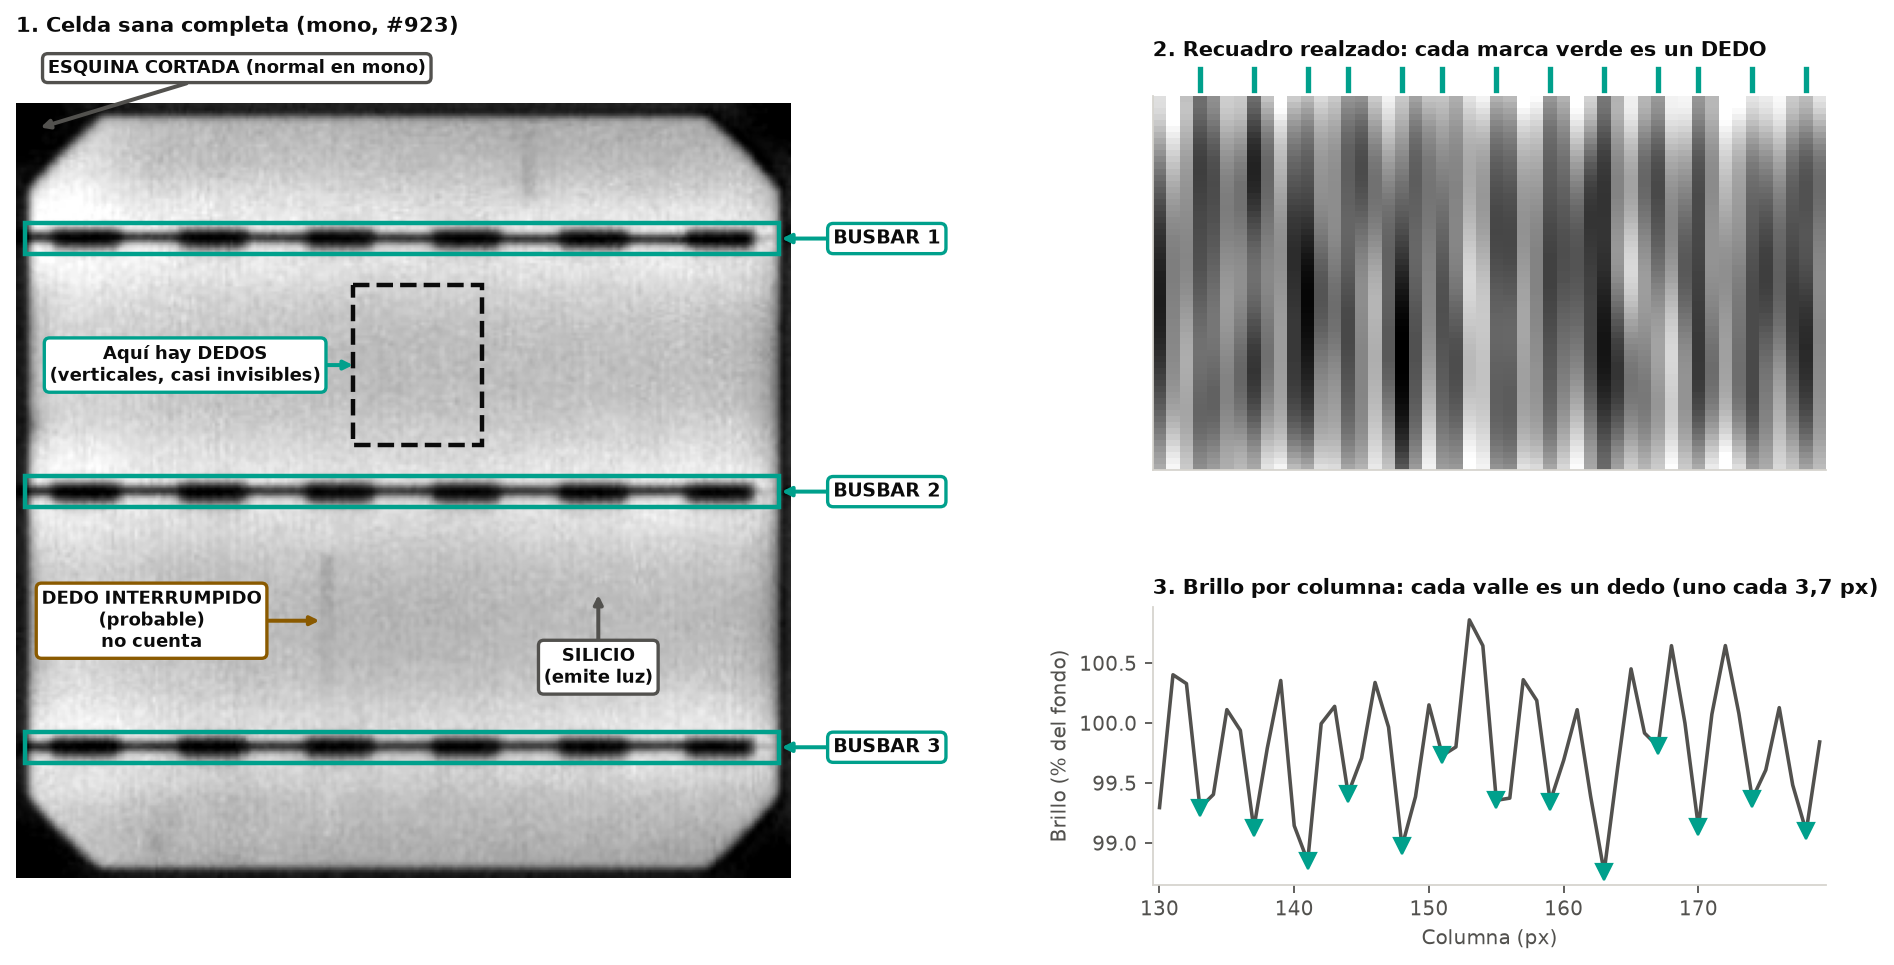
\includegraphics[height=0.66\textheight]{b0a_anatomia_celda.png}

  \raggedright\small
  El metal es oscuro porque no emite luz. Si no se quita, el filtro de grietas lo marca: miles de píxeles en una celda sana.
\end{frame}

\begin{frame}{Las dos técnicas}{3 · Métodos}
  \begin{columns}[t]
    \begin{column}{0.47\textwidth}
      \cab{A · Notch gaussiano (lab 9)}
      \footnotesize $I_A=\mathcal{F}^{-1}\{H\,F\}$, agujeros en $(0,\pm k v_0)$, $v_0=300/P$ por celda. $\sigma_n=1$, lo más ancho que los mantiene
      separados; $K=24$. En toda la celda (\textbf{A-global}) o solo en las filas de busbar (\textbf{A-filas}).
    \end{column}
    \begin{column}{0.47\textwidth}
      \cab{B · Cierre morfológico (lab 10)}
      \footnotesize $I_B=(I_n\oplus B)\ominus B$, elemento vertical de $h=21$ px, más alto que la banda ($\approx$8 px), solo en las filas de busbar.
      $h$ dio el menor resto por tramos.
    \end{column}
  \end{columns}
  \vspace{0.15cm}
  \centering
  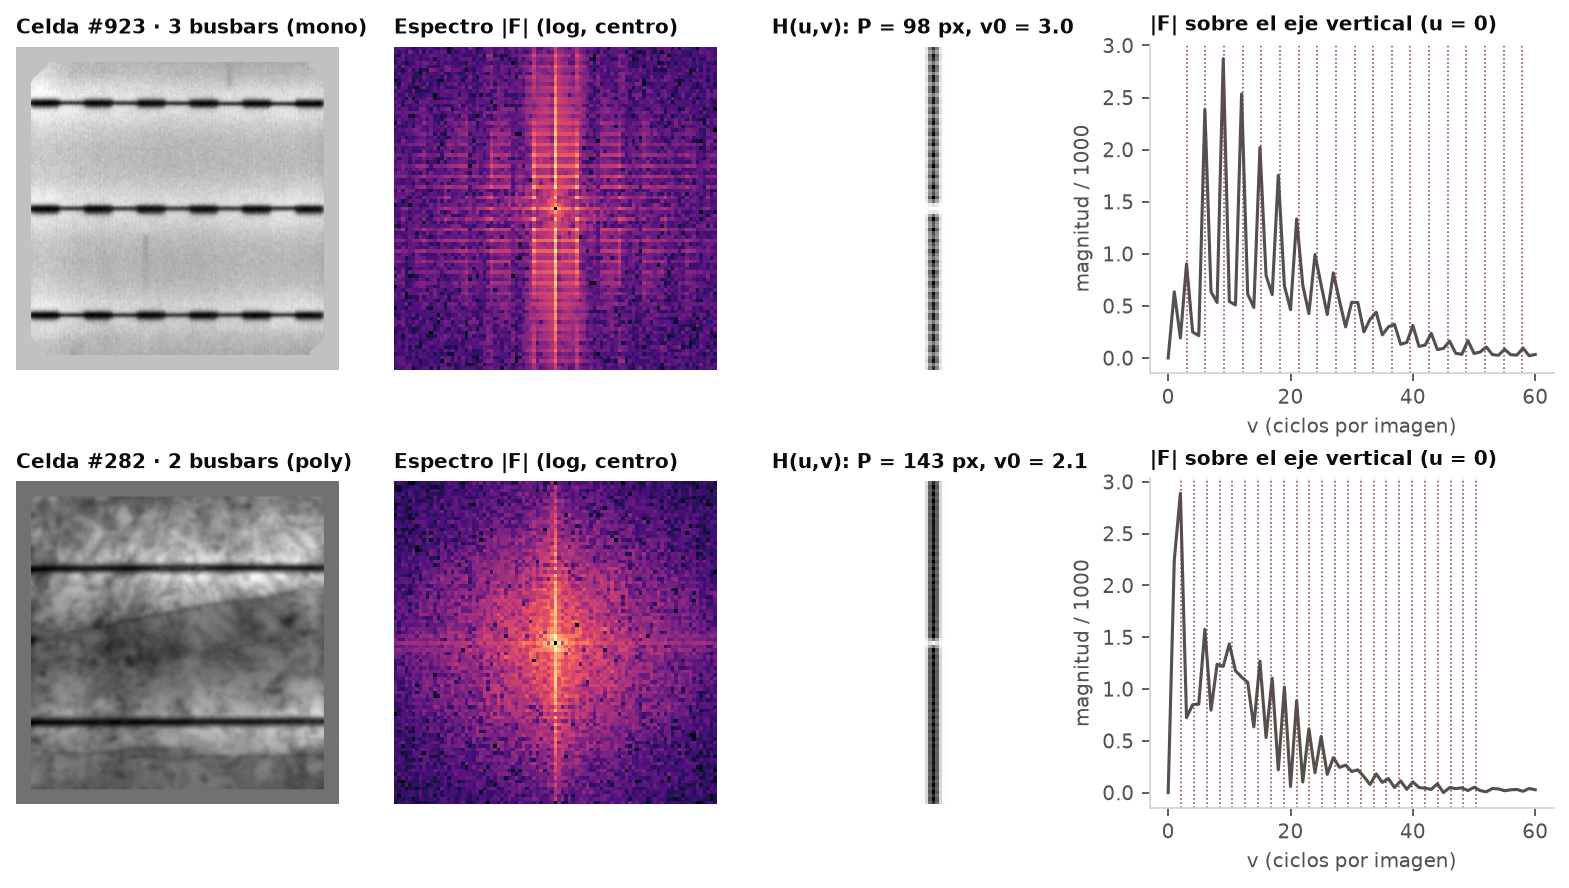
\includegraphics[height=0.36\textheight]{b1_espectro_notch.png}

  \footnotesize Parámetros fijados en entrenamiento. Todo lo que sigue se mide en \textbf{validación}.
\end{frame}

\begin{frame}{Primero había que encontrar los busbars}{4 · Resultados · Detección}
  \centering
  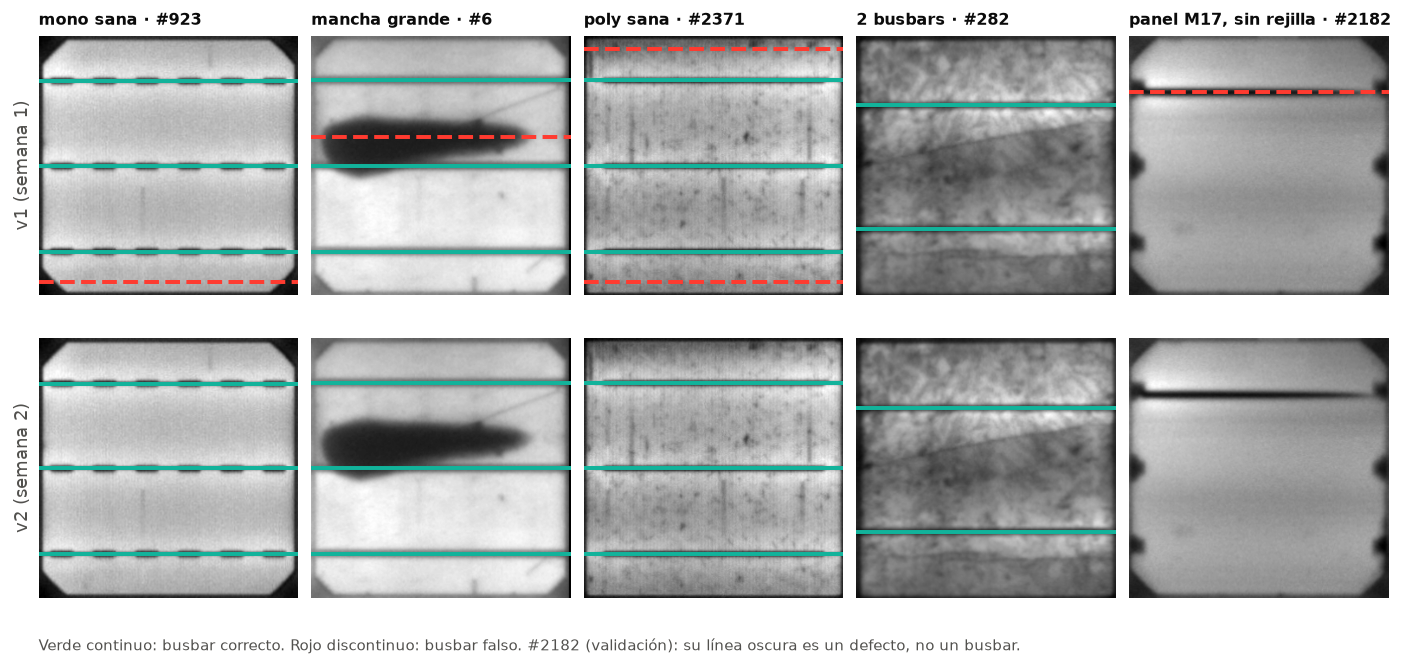
\includegraphics[width=0.78\textwidth]{b5_deteccion_v1_v2.png}

  \raggedright\small
  Rejilla exacta en validación: \textbf{11,8\,\%} con v1 y \textbf{100\,\%} con v2. Referencia: lectura de la imagen mediana de cada panel.
  \textbf{Hallazgo:} las 72 celdas del panel M17 (validación) no tienen busbars al frente.
\end{frame}

\begin{frame}{Antes y después}{4 · Resultados · Imágenes}
  \centering
  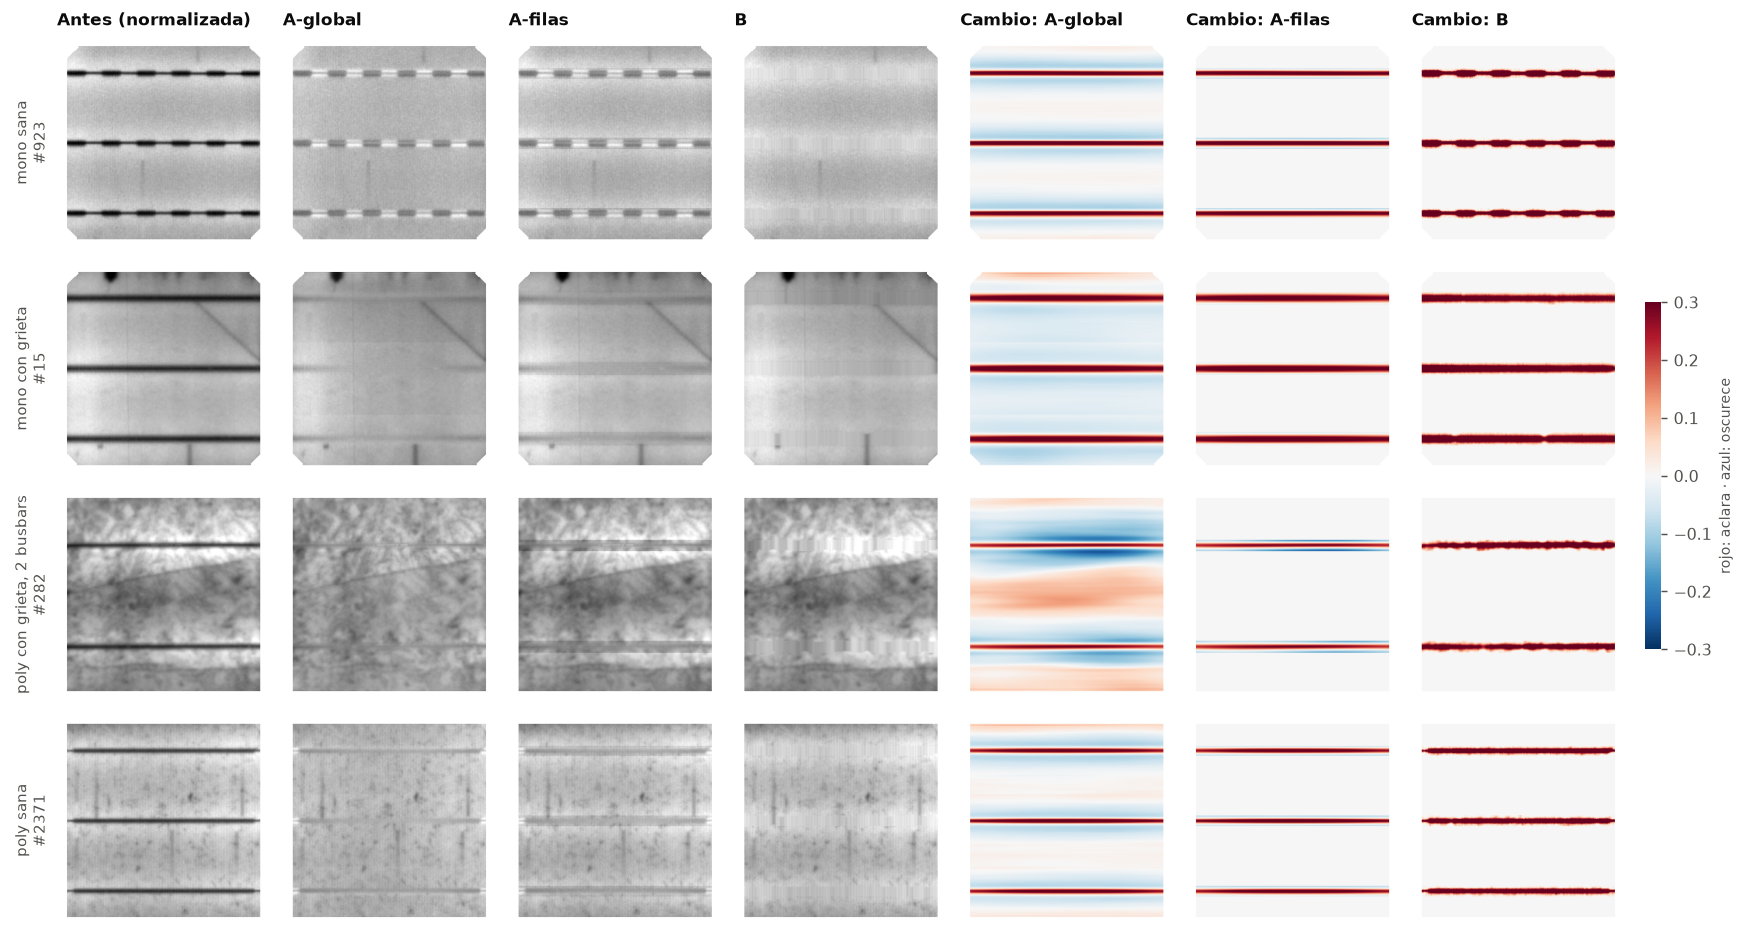
\includegraphics[height=0.74\textheight]{b2_antes_despues.png}
\end{frame}

\begin{frame}{Criterios de la tabla 3 en validación}{4 · Resultados · 360 celdas con rejilla}
  \centering\footnotesize
  \begin{tabular}{@{}l ccc c c c@{}}
    \toprule
    & \multicolumn{3}{c}{1 · Resto} & 2 · Fuera & 4 · Tiempo & 3 · AUC CNN \\
    \cmidrule(lr){2-4}
    & todas & mono & poly & todas & ms/celda & (decide) \\
    \midrule
    Sin tocar & 40,3\,\% & 41,4\,\% & 39,7\,\% & 0 & – & semana 3 \\
    A-global & 5,9\,\% & 6,1\,\% & 5,9\,\% & 3,4\,\% & 8,5 & semana 3 \\
    A-filas & 11,7\,\% & 11,6\,\% & 11,8\,\% & 0 & 9,5 & semana 3 \\
    B & \textbf{\color{ud}0,9\,\%} & 1,1\,\% & 0,8\,\% & 0 & \textbf{\color{ud}0,8} & semana 3 \\
    \bottomrule
  \end{tabular}

  \vspace{0.3cm}
  \raggedright
  \begin{itemize}
    \item El notch deja la banda a medias cuando el busbar es punteado: esa energía cae fuera del eje vertical.
    \item A-global altera el brillo de toda la celda. A-filas y B no tocan nada fuera de las bandas, por construcción.
    \item B gana los tres criterios de apoyo. Eso todavía no lo hace el elegido.
  \end{itemize}
\end{frame}

\begin{frame}{Cada método borra un tipo distinto de grieta}{4 · Resultados · Grietas sintéticas (apoyo)}
  \centering
  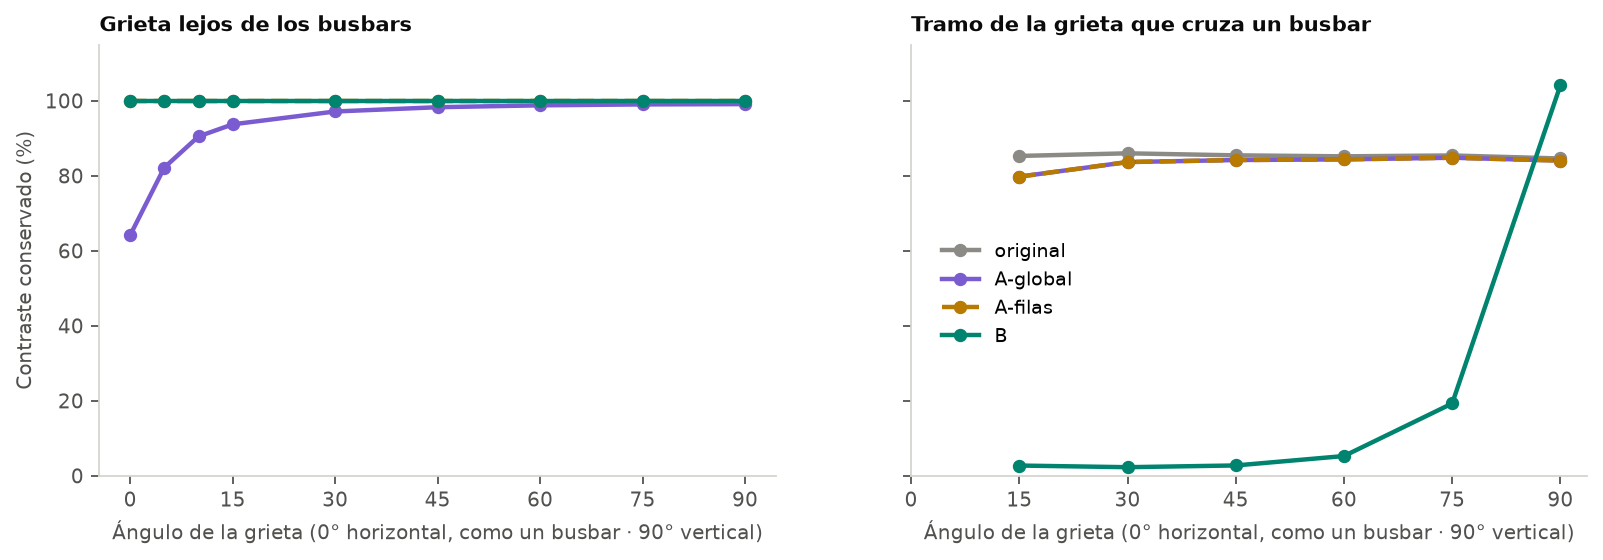
\includegraphics[width=0.92\textwidth]{b6_grietas_por_angulo.png}

  \raggedright\small
  El notch global debilita las horizontales un 36\,\%. El cierre borra el tramo que cruza la banda, salvo en las verticales.
  Por eso el criterio 3 puede contradecir a los otros tres.
\end{frame}

\begin{frame}{Quitar los dedos no conviene}{4 · Resultados · Dedos y grietas verticales}
  \centering
  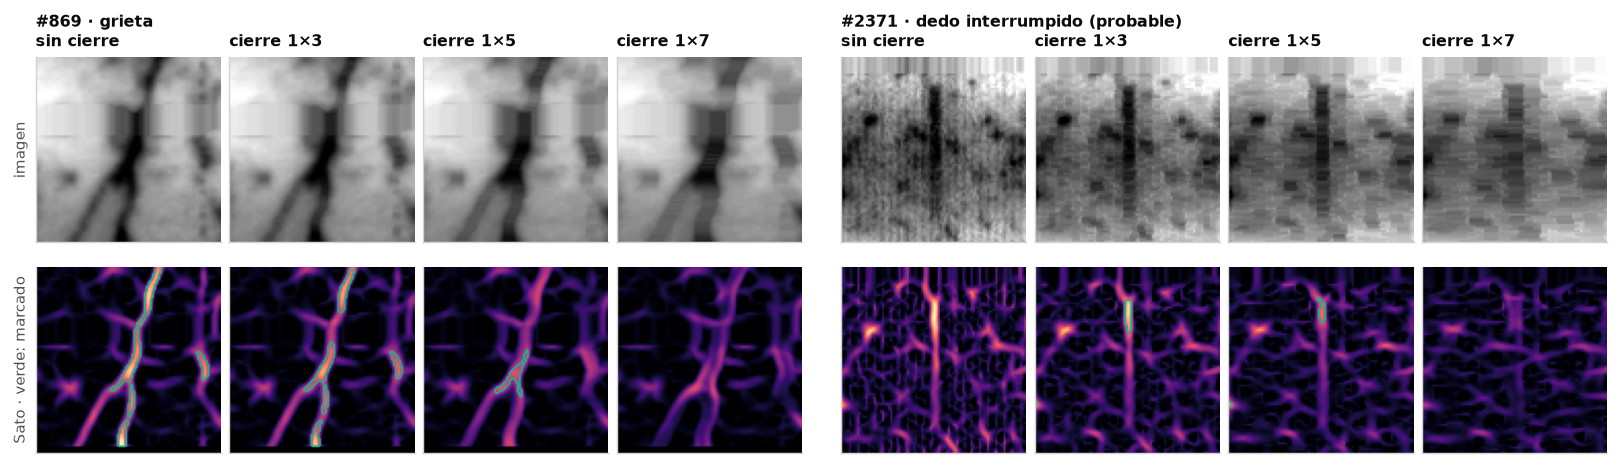
\includegraphics[width=0.92\textwidth]{b4_grietas_verticales.png}

  \vspace{0.1cm}
  \begin{columns}[c]
    \begin{column}{0.5\textwidth}
      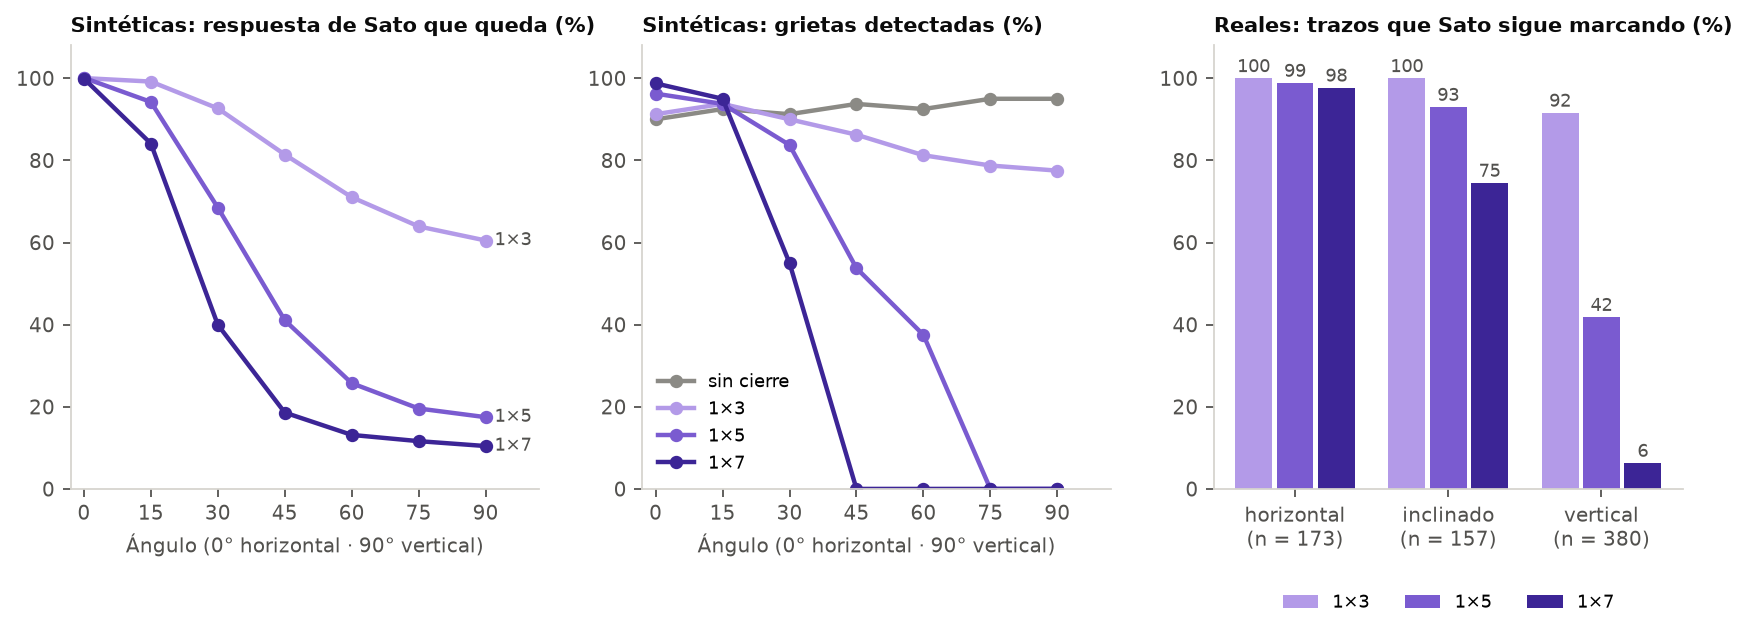
\includegraphics[width=\linewidth]{b4b_sato_dedos.png}
    \end{column}
    \begin{column}{0.47\textwidth}
      \scriptsize
      \begin{itemize}
        \item \textbf{Sin beneficio:} la falsa grieta en mono sube de 89 a 119 px ($1\times3$); en poly baja un 12\,\% solo con $1\times5$.
        \item \textbf{$1\times5$ y $1\times7$, descartados:} ninguna vertical fina se detecta.
        \item \textbf{$1\times3$:} Sato pierde un 40\,\% en verticales finas sintéticas y un 9\,\% en 380 trazos reales.
      \end{itemize}
    \end{column}
  \end{columns}
\end{frame}

\begin{frame}{Decisiones, riesgos y semana 3}{5 · Decisiones · 6 · Riesgos · 7 · Plan}
  \begin{columns}[t]
    \begin{column}{0.31\textwidth}
      \cab{Decidimos}
      \footnotesize
      \begin{itemize}
        \item Detección v2 desde ahora. La línea base del Avance 1 no se toca.
        \item Proponemos no quitar los dedos (cambia §4.3). Lo confirma la CNN.
        \item Mono con y sin M17.
      \end{itemize}
      {\color{ud}\bfseries Sin cambios al alcance.} La prueba no se ha usado.
    \end{column}
    \begin{column}{0.31\textwidth}
      \cab{Vigilamos}
      \footnotesize
      \begin{itemize}
        \item La referencia de la detección es lectura nuestra; validación no es del todo a ciegas.
        \item M17: la CNN no verá celdas sin rejilla al entrenar.
        \item Dedos interrumpidos: parecen grietas.
        \item Granos de poly.
      \end{itemize}
    \end{column}
    \begin{column}{0.31\textwidth}
      \cab{Semana 3}
      \footnotesize
      \begin{itemize}
        \item Mapas de grietas (Sato; Gabor en poly) y de zonas apagadas.
        \item CNN con \textbf{A}, con \textbf{B} y con la original, tres semillas. B con y sin dedos.
        \item \textbf{Elegir con el criterio 3} y congelar.
      \end{itemize}
    \end{column}
  \end{columns}
  \vspace{0.25cm}
  \footnotesize\textbf{Demo:} \texttt{entregas/avance\_2/web/laboratorio\_busbars.html} aplica el notch y el cierre en vivo sobre seis celdas reales.
\end{frame}

{\setbeamercolor{background canvas}{bg=ud}
\begin{frame}[plain]
  \begin{tikzpicture}[remember picture,overlay]
    \node[anchor=north west] at ([xshift=0.6cm,yshift=-0.35cm]current page.north west)
      {
\includegraphics[height=1.15cm]{logo_blanco.png}};
  \end{tikzpicture}
  \centering\color{white}
  \vspace{1.2cm}
  {\Huge Preguntas}\par\vspace{0.4cm}
  {\large\itshape Cifras: \texttt{reports/metricas/semana2\_*.json}}\par\vspace{0.8cm}
  {\footnotesize S. Deitsch \emph{et al.}, «Automatic classification of defective photovoltaic module cells in electroluminescence images»,
  \emph{Solar Energy}, vol. 185, 2019. · Imágenes ELPV, CC BY-NC-SA 4.0.}
\end{frame}}

\end{document}
